\scanpage{8}

\uline{Corollaire.} Cet ouv est dense ssi pour \unsure{tt|tout} pt \uline{maximal} $x\in X$, $\underline O_{X,x}$ est réduit et $k(x)$ est une extension \uline{séparable} de $k$ $[\Leftrightarrow$ \inserted{\unsure{au cas une|au cas d'une} ext. de t. f.} extension étale d'une extension \unsure{transcend.te|transcendante|transcend. ou} pure$]$

\uline{Corollaire} Si $k$ est parfait, l'ens des pts où $X$ est lisse est un ouvert dense.

\uline{NB} On a un \unsure{réslt|rés\textsuperscript{t}} analogue pour la \uline{normalité géométrique}, sans condition de finitude. Si $X$ est \deleted{\unsure{géom normal|géom norm}} \inserted{loc de} t. f. sur $k$, l'ens des pts où $X$ est géom normal sur $k$ est ouvert, \inserted{et dense si $k$ est parfait} [Une extension d'un corps est géom normale ssi elle est séparable)

\figure{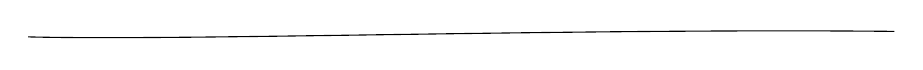
\begin{tikzpicture}\draw (0,0) .. controls (2,-.05) and (7,.11) .. (11,.07);\end{tikzpicture}}

\uline{Proposition} $G$ groupe sur corps $k$. Conditions équivalentes

\margin{marche aussi si $X$ un \deleted{\unsure{gpe|esp.}} \inserted{schéma} sur lequel $G$ opère et tel que \deleted{$G\times X\xrightarrow{\unsure{\pi|p}} X$} $G\times X\longrightarrow X\times X$ surjectif $(g,x)\longmapsto(gx,x)$ ($X$ essentiellement homogène)}% slanted

a) $G$ \deleted{\unsure{géom norm|géom. normal}} séparable $/k$ en un pt \qquad a$'$) $G$ sép. $/k$ \deleted{en un point}

b) $G$ géom normal sur $k$

c) (Si $G$ loc de t. f. sur $k$) $G$ lisse $/k$

On a évidemment \inserted{c $\Rightarrow$} b) $\Rightarrow$ a$'$) $\Longrightarrow$ a) \deleted{$\Longrightarrow$ \unsure{b)|b)?}}.

\margin{\uline{NB} Si $G$ de t. f. sur $k$, alors $G$ \deleted{\unsure{re|ré}} \unsure{réduit|reduit} $\Rightarrow G$ sép.? \deleted{(\unsure{est-ce que|et si pas|est-ce} le \unsure{$k$|$h$} \unsure{est} \unsure{stable dans|étant donné}}}% slanted

a) $\Rightarrow$ b) \qquad Soit $g\in G$, \deleted{un} pt maximal de $G$. \deleted{\unsure{géom|gén.}} \deleted{pour que $g$ \unsure{$G$ est géom normal en $g$|soit géom il suffit que $g$},} Alors $k(g)$ est une ext. séparable de $k$, donc $G$ est géom normal en $g$. \deleted{Donc, quitte \unsure{à faire une extension|à une extension} par descente on est ramené à \unsure{voir le cas|voir l'assert} pour $g$ rat. sur $k$.} \deleted{Soit $g'$ un pt maximal de $G$, on sait que $G$ est géom normal en $g'$; faisant une extension} Donc $G$ a \uline{un} pt $g$ où il est géom. normal. Prouvons qu'il en est de $=$ pour tt autre pt $g'$. Par ext. de la base, on est ramené au cas où $g$, $g'$ rat $/k$. Mais alors ils sont conjugués par translation !

b) $\Rightarrow$ a) \qquad \unsure{Esq.|Est.} en démonstration.

\uline{Corollaire 1} Soit $k$ parfait. Alors $G_{\text{\unsure{red|réd}}}$ est géom normal \unsure{$\bar k$|$k$|$\bar B$} (resp. lisse, si $G$ est loc. de t. f. sur $k$)

% archive sheet number: 7

